\section{Auswertung}

\subsection{Quarzkügelchen}
    Für die weitere Auswertung ist es fundamental die Auflösung der aufgenommen Bilder zu kennen.
    Zu diesem Zweck wird die Größe eines Pixels in der CCD-Kamera-Software bestimmt.
    Die Größe der verwendeten Quarzkügelchen ist mit \qty{2,06}{\um} bekannt.
    Befindet sich nun ein Quarzkügelchen im Fokus des Mikroskops bzw. der Falle, wird es mit dem Zeichenwerkzeug markiert, siehe \autoref{fig:Pixelgroesse}.
    \begin{figure}[ht]
        \centering\captionsetup{format=plain}
        \includegraphics[width=0.5\textwidth]{bilder/Pixelgröße.JPG}
        \caption{Markierung eines eingefangenen Quarzkügelchens im Fokus des Mikroskops zur Bestimmung der Größe eines Pixels.}
        \label{fig:Pixelgroesse}
    \end{figure}
    \FloatBarrier
    Nach dem Zählen der Pixel entlang des Durchmessers des gelben Kreises ergibt sich die Pixelgröße zu
    \begin{equation}
        \mathrm{Pixelgröße} = \frac{\SI{2,06}{\um}}{122} \approx \SI{16,9}{\nm} \;.
    \end{equation}

\subsection{Kalibrierung der Spannung der Viersegment-Photodiode}
    Den Quarzkugeln wird NaCl-haltiges Wasser beigemischt.
    Die Kationen schirmen die elektrische Ladung der negativ geladenen Kugel ab, was ein Festkleben an den Wänden der Probenkammer wahrscheinlicher macht.
    Nun ist es möglich Messungen durchzuführen ohne, dass sich die Quarzkugeln bewegen.

    Zur Umrechnung des Spannungssignals der Viersegment-Photodiode in die tatsächliche Position in der Fokusebene des Mikroskops wurde die Optische Pinzette in x- und y-Richtung über eine fixierte Quarzkugel gescannt.
    Dabei wurde das auf der Photodiode gemessene Spannungssignal gegen die Position aufgetragen.
    Dies wurde für mehrere Laserleistungen durchgeführt, hier wird die Vorgehensweise exemplarisch nur für \qty{200}{mA} gezeigt.
    An den in \autoref{fig:PosCal_200mA} zu sehenden S-Kurven zwischen den blauen Linien wurden lineare Regressionen durchgeführt, um die Steigungen zu bestimmen.
    Diese geben die Konversationsfaktoren zwischen Photodiodenspannung und Position an.

    \begin{figure}[ht]
        \centering\captionsetup{format=plain}
        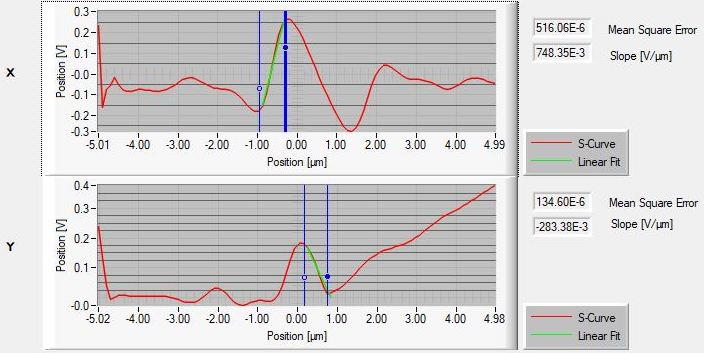
\includegraphics[width=0.6\textwidth]{bilder/PosCal_200mA.JPG}
        \caption{Ein Screenshot aus dem Thorlabs Programm im Menüpunkt \glqq \textit{position calibration} von einem Scan über eine fixierte Quarzkugel. Die Steigung der Flanken wird durch die grüne Gerade gefittet und gibt den Konversationsfaktor zwischen Photodiodenspannung und Position an.}
        \label{fig:PosCal_200mA}
    \end{figure}
    \FloatBarrier
    Trägt man die Konversationsfaktoren für verschiedene Laserleistungen auf, so ist kein deutlicher Trend zu erkennen.
    Es ist jedoch möglich die durchschnittlichen Konsversationsfaktoren für die x- und y-Richtung zu bestimmen:
    \begin{equation*}
        m_{\mathrm{x,konv}} \approx \qty{0,71}{V m^{-1}} \qquad m_{\mathrm{y,konv}} \approx \qty{0,29}{V m^{-1}}
    \end{equation*}
    \begin{figure}[ht]
        \centering\captionsetup{format=plain}
        \includegraphics[width=0.6\textwidth]{plots/Konversionsfaktoren.pdf} \vspace*{-0.5cm}
        \caption{Hier sind die Konversationsfaktoren für verschiedene Laserleistungen aufgetragen.}
        \label{fig:Konversionsfaktoren}
    \end{figure}
    \FloatBarrier
    Das in der Viersegment-Photodiode ankommende Summensignal, welches proportional zur einfallenden Gesamtintensität ist wird zur Bestimmung der Position der Probenoberfläche genutzt.
    Dabei wird die axiale Position der Probenoberfläche relativ zum Fokus der Falle mit dem z-Piezo variiert.
    Der Ursprung der in \autoref{fig:Diodensumme} auf der x-Achse aufgetragene z-Position wurde zufällig gewählt.
    Durch einen Vergleich mit der Theorie lässt sich die relative Position der Probenoberfläche grob bestimmen zu ca. \qty{33}{\um}.
    \begin{figure}[ht]
        \centering\captionsetup{format=plain}
        \includegraphics[width=0.6\textwidth]{plots/Diodensumme.pdf} \vspace*{-0.5cm}
        \caption{Zur Bestimmung der Position der Probenoberfläche wird das Diodensummensignal als Funktion der axialen Position der Probe und damit als Funktion der Position einer fixierten Quarzkugel gemessen.}
        \label{fig:Diodensumme}
    \end{figure}
    \FloatBarrier

\subsection{Fallensteifigkeit, Boltzmann-Konstante, Stokes'sche Fallenkraft}
    Zur Bestimmung der Fallensteifigkeit werden Zeitserien der x- und y-Position einer Quarzkugel über eine Kalibrierungsdauer von $\Delta t_{\mathrm{cal}} = \qty{1}{s}$ aufgenommen.
    An der daraus bestimmten spektralen Leistungsdichte PSD kann eine Lorentzfunktion
    \begin{equation*}
        \mathrm{PSD}(f) = \frac{A}{f^2 + f_0^2}
    \end{equation*}
    gefittet werden wie in \autoref{fig:PSD_keineKraft} zu sehen, die einen Wert für die sogenannte Roll-Off-Frequenz $f_0$ angibt.
    Aus dieser wiederum ergibt sich die Fallensteifigkeit
    \begin{equation*}
        k = 2 \pi \beta f_0 \quad \mathrm{mit} \quad \beta = 3 \pi \eta d \,,
    \end{equation*}
    wobei $\eta = \qty{8,9e-4}{Pa s}$ die Viskosität des fluiden Mediums und $d=\qty{2,06}{\um}$ der Durchmesser der Quarzkugeln ist.
    Dieses Verfahren ist exemplarisch an der \autoref{fig:pos_keineKraft, fig:k_keineKraft} und \ref{fig:k_keineKraft} für einen Laserstrom von \qty{150}{mA} verdeutlicht.
    \begin{figure}[ht]
        \centering\captionsetup{format=plain}
        \includegraphics[width=0.8\textwidth]{plots/pos_keineKraft.pdf} \vspace*{-0.5cm}
        \caption{.}
        \label{fig:pos_keineKraft}
    \end{figure}
    \begin{figure}[ht]
        \centering\captionsetup{format=plain}
        \includegraphics[width=0.8\textwidth]{plots/PSD_keineKraft.pdf} \vspace*{-0.5cm}
        \caption{.}
        \label{fig:PSD_keineKraft}
    \end{figure}
    \begin{figure}[ht]
        \centering\captionsetup{format=plain}
        \includegraphics[width=0.6\textwidth]{plots/k_keineKraft.pdf} \vspace*{-0.5cm}
        \caption{.}
        \label{fig:k_keineKraft}
    \end{figure}
    \FloatBarrier

\subsection{Vesikel in Zwiebelzellen}

